\chapter{Аналитическая часть}

\section{Описание объектов сцены}

Сцена состоит из следующих объектов: камера, источник света, пол, имеющий структуру, и слайм.

Камера представляет собой невидимый объект, содержащий в себе информацию о координатах положения камеры в пространстве и векторе направления взгляда и использующийся для получения изображения на дисплее.

Источник света представляет собой материальную точку, которая испускает лучи света во все стороны. Данный объект хранит в себе информацию о координатах положения в пространстве источника света и цвете.

Пол представляет собой плоскость, заданную уравнением $z = 0$. Предполагается, что все объекты находятся над полом или на нем.

Слайм - это моделируемая игрушка <<Лизун>>. В нашей программе слайм представляет собой вязкоупругое тело. При отсутствии внешних сил слайм имеет форму шара.

\section{Выбор модели представления объекта}

Для задания трехмерных моделей выделяют три формы: каркасную, поверхностную и объемную.

\subsection{Каркасная модель}
Каркасная модель является простейшим видом. В ней задается информация о вершинах и ребрах объекта. Однако, ввиду своей простоты, данный вид обладает серьезным недостатком: не всегда корректно передается представление об объекте.

\subsection{Поверхностная модель}
Поверхностная модель предполагает хранение информации не только о вершинах и ребрах объекта, но и о его поверхности. Поверхность может быть описана как аналитически, так и с помощью задания участков поверхности как поверхностей того или иного рода. Недостатком данной модели является невозможность определения, с какой стороны поверхности находится материал объекта.

\subsection{Объемная модель}
Объемная модель отличается от поверхностной лишь тем, что в ней мы храним информацию о расположении материала объекта, указывая направление вектора внутренней нормали

Для данного проекта была выбрана поверхностная модель, так как каркасная модель не всегда правильно передает представление об объекте, а объемная модель является избыточной в рамках решаемой задачи.

\section{Выбор модели представления поверхности объекта}

Поверхность объекта может быть описана как аналитически, так и с помощью полигональной сетки. В аналитическом методе поверхность объекта рассматривается как множество точек, координаты которых удовлетворяют заданному уравнению, в то время как полигональная сетка представляет собой совокупность вершин, ребер и полигонов, соединенных таким образом, что каждое ребро принадлежит не более, чем двум многоугольникам.

Существует несколько способов описания полигональных сеток:

\begin{enumerate}
	\item список вершин;
	\item список ребер;
	\item список граней.
\end{enumerate}

Первый способ подразумевает хранение информации о сетке в виде перечня координат вершин, в котором каждая вершина записывается один раз в виде тройки координат. При этом каждый многоугольник задается множеством порядковых номеров вершин в списке.

Во втором способе базовую информацию дает список вершин, но многоугольники описываются ссылками на список ребер, в котором каждое из них упоминается только один раз. В свою очередь, ребра представляются в виде пары граничных вершин и перечня смежных многоугольников, число которых не превышает двух.

В третьем способе хранятся список вершин и список граней. В каждой грани хранится информация о трех вершинах.

Для данного проекта была выбрана модель полигональной сетки, ввиду простоты реализации и отсутствия серьезных проблем при описании сложных объектов. Кроме того, хранение информации о сетке будет осуществляться с помощью списка граней, так как данный способ предоставляет полную информацию о гранях, которая может быть крайне полезна при реализации алгоритмов удаления невидимых ребер и поверхностей.

\section{Выбор метода физического моделирования объекта}

Для моделирования процессов, протекающих при деформации слайма, необходимо выбрать соответствующий метод описания физических свойств тела.

Существует три метода моделирования деформируемых тел:

\begin{enumerate}
	\item метод конечных элементов;
	\item метод граничных элементов;
	\item метод с использованием модели масс с пружинами.
\end{enumerate}

\subsection{Метод конечных элементов}
В данном методе объект разбивается на конечные элементы, соединяющиеся
между собой в узлах. Каждый конечный элемент должен быть достаточно
простым, чтобы имелась возможность легко определить напряжения в любой его части по заданным перемещениям узлов. По точкам составляется система уравнений, которая решается относительно перемещений рассматриваемых точек. Данная модель имеет высокую точность, однако требует знания характеристик материала объекта, необходимых для рассчета соотношений для каждого элемента.

\subsection{Метод граничных элементов}
Метод граничных элементов является интересной альтернативой метода
конечных элементов, так как все преобразования осуществляются над точками
поверхности объекта, что дает прирост к скорости вычислений. Основная
сложность реализации данного метода заключается в преобразовании
интегральной формы уравнения движения тела в поверхностный интеграл.

\subsection{Модель масс с пружинами}
Система масс с пружинами подразумевает хранение объекта, как совокупности точечных масс, соединенных между собой сетью невесомых пружин.

Для описания динамики движения слайма была выбрана модель масс с
пружинами, так как она позволяет выполнять простые вычисления и дает
приемлемую точность моделирования.

\section{Выбор алгоритма удаления невидимых ребер и поверхностей}

Рассмотрим следующие алгоритмы удаления невидимых ребер и поверхностей:

\begin{itemize}
	\item алгоритм Робертса;
	\item алгоритм Варнока;
	\item алгоритм, используюший z-буфер;
	\item алгоритм обратной трассировки лучей.
\end{itemize}

\subsection{Алгоритм Робертса}

Алгоритм Робертса работает в объектном пространстве, осуществляя
удаление невидимых линий выпуклых тел. Выполнение данного алгоритма можно
разделить на 4 этапа:

\begin{enumerate}
	\item подготовка исходных данных;
	\item удаление ребер, экранируемых самим телом;
	\item удаление ребер, экранируемых другими телами;
	\item удаление линий пересечения тел, экранируемых самими телами и другими телами, связанными отношением протыкания.
\end{enumerate}

На первом этапе для каждого тела формируется матрица, каждый столбец
которой содержит коэффициенты уравнения плоскости:
\begin{equation}\label{plane_eq}
	ax + bx + cz + d = 0,
\end{equation}
проходящей через соответствующую грань. Данная матрица имеет вид:
$$
V =
\begin{pmatrix}
	a_1 & a_2 & \cdots & a_n \\
	b_1 & b_2 & \cdots & b_n \\
	c_1 & c_2 & \cdots & c_n \\
	d_1 & d_2 & \cdots & d_n \\
\end{pmatrix},
$$
где $a_i$, $b_i$, $c_i$ и $d_i$ - коэффициенты уравнения~\eqref{plane_eq} $i$-ой плоскости.

Матрица тела должна быть сформирована корректно. Это значит, что любая
точка, лежащая внутри тела, должна лежать по положительную сторону от каждой
грани тела. Если для какой-либо грани это условие не выполняется,
соответствующий столбец матрицы умножается на -1.

На втором этапе указывается расположение наблюдателя и направление его
взгляда. Как правило, наблюдатель располагается в бесконечности на
положительной полуоси z и смотрит в сторону начала координат. В однородных
координатах вектор такого направления равен:
$$
	E = [0, 0, -1, 0].
$$

Для определения невидимых граней нужно умножить вектор $E$ на матрицу $V$. Отрицательные компоненты результирующего вектора соответствуют
невидимым ребрам тела.

На третьем этапе работы алгоритма для определения невидимых линий
строится луч, соединяющий точку наблюдения с точкой на ребре. Точка невидима,
если луч проходит через тело.

На четвертом этапе ведется поиск ребер, образовавшихся в результате
взаимного протыкания тел. Вновь полученные ребра проверяются на
экранирование телами.

Алгоритм Робертса дает высокую точность вычислений, однако сложен в
реализации.

\subsection{Алгоритм Варнока}

Данный алгоритм работает в пространстве изображений. В пространстве
изображения рассматривается окно и решается вопрос о том, пусто ли оно, или его
содержимое достаточно просто для визуализации. Если это не так, то окно
разбивается на фрагменты до тех пор, пока содержимое подокна не станет достаточно простым для визуализации или его размер не достигнет требуемого
предела разрешения.

Конкретная реализация алгоритма Варнока зависит от метода разбиения
окна и от критериев, используемых для того, чтобы решить, является ли
содержимое окна достаточно простым. В оригинальной версии алгоритма Варнока
каждое окно разбивается на четыре одинаковых подокна. Окно является пустым,
когда все многоугольники сцены являются внешними по отношению к этому окну.
Пределом разбиения является размер окна в 1 пиксель. Тогда определяем глубину
каждого из рассматриваемых многоугольников в этой точке и изображаем точку
многоугольника, наиболее близкого к пользователю.

Алгоритм Варнока прост в реализации, однако возможны большие затраты по
времени, если рассматривается область с большим количеством информации.

\subsection{Алгоритм, используюший z-буфер}

Данный алгоритм работает в пространстве изображений. В нем
используются буфер кадра и z-буфер. Буфер кадра используется для запоминания
интенсивности каждого пиксела в пространстве изображения, в то время как z-
буфер — это отдельный буфер глубины, используемый для запоминания глубины
(координаты z) каждого видимого пиксела в пространстве изображения.

В процессе работы значение z каждого нового пикселя, который нужно
занести в буфер кадра, сравнивается с глубиной того пиксела, который уже занесен
в z-буфер. Если это сравнение показывает, что новый пиксел расположен впереди
пиксела, находящегося в буфере кадра, то новый пиксел заносится в этот буфер, и
производится корректировка z-буфера новым значением z. Если же сравнение дает
противоположный результат, то никаких действий не производится.

Главное преимущество алгоритма — простота. Кроме того, этот алгоритм
решает задачу об удалении невидимых поверхностей и делает тривиальной
визуализацию пересечений сложных поверхностей. Однако, несмотря на свою
простоту, алгоритм требует использование большого объема памяти. Кроме того,
недостаток алгоритма заключается еще в трудоемкости реализации эффектов
прозрачности.

\subsection{Алгоритм обратной трассировки лучей}

Основная идея, лежащая в основе трассировки лучей, заключается в том, что
наблюдатель видит любой объект посредством испускаемого неким источником
света, который падает на объект и затем каким-то путем доходит до наблюдателя
согласно законам оптики. Однако не все лучи света доходят до наблюдателя, что
делает процесс отслеживания этих лучей вычислительно неэффективным.
Поэтому лучше отслеживать лучи в обратном направлении, то есть от наблюдателя
к объекту, причем испуская лучи от точки наблюдателя через каждый пиксел
экрана.

Для данной работы был выбран алгоритм обратной трассировки лучей, так
как он, несмотря на малую производительность из-за большого количества
вычислений, позволяет получить реалистичное изображение с учетом оптических
явлений, таких как отражение и преломление.

\section{Выбор модели освещения}

Построение реалистических изображений включает в себя как физические,
так и психологические процессы. В частности, при визуализации сцены
учитываются законы оптики: отражение, преломление, поглощение света и т. д.
Поэтому необходимо выбрать модель освещения для построения изображения.

\subsection{Модель Ламберта}

Модель Ламберта описывает диффузное освещение. Модель показана на рисунке \ref{lambert}.

\begin{figure}[H]
	\centering
	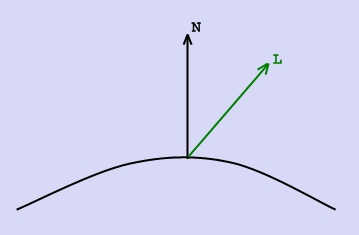
\includegraphics[width=0.6\linewidth]{lambert}
	\caption{Модель освещения Ламберта}
	\label{lambert}
\end{figure}

Cвет точечного источника диффузно отражается от идеальной поверхности по закону косинусов Ламберта: интенсивность отраженного света пропорциональна косинусу угла между направлением света L и нормалью к поверхности N:
\begin{equation}\label{lambert_eq}
	I = I_l k_d cos \theta,
\end{equation}
где $I$ - интенсивность отраженного света,\\
\text{~~~~~}$I_l$ - интенсивность точечного источника в направлении L,\\
\text{~~~~~}$k_d$ - коэффициент диффузного отражения,\\
\text{~~~~~}$\theta$ - угол между направлением света L и нормалью к поверхности n, $0~\le~\theta~\le~\frac{\pi}{2}$

\subsection{Модель Фонга}

Модель Фонга — это классическая модель освещения, представляющая
собой совокупность диффузной и зеркальной составляющих. Модель представлена на рисунке \ref{phong}.

\begin{figure}[H]
	\centering
	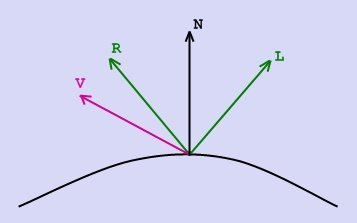
\includegraphics[width=0.6\linewidth]{phong}
	\caption{Модель освещения Фонга}
	\label{phong}
\end{figure}

Работает модель
таким образом, что кроме равномерного освещения на материале могут появляться
блики. Местонахождение блика на объекте определяется из закона равенства углов
падения и отражения. Чем ближе наблюдатель к углам отражения, тем выше
яркость соответствующей точки.

Зеркальная модели составляющая описывается выражением:

\begin{equation}\label{phong_ref_eq}
	I = I_l w(i, \lambda) cos^n \alpha,
\end{equation}
где $I$ - интенсивность отраженного света,\\
\text{~~~~~}$I_l$ - интенсивность точечного источника в направлении L,\\
\text{~~~~~}$w(i, \lambda)$ - кривая отражения, представляющая отношение зеркально отраженного света к падающему как функцию угла падения $i$ и длины волны $\lambda$;\\
\text{~~~~~}$n$ - степень, аппроксимирующая пространственное распределение зеркально отраженного света;\\
\text{~~~~~}$\alpha$ - гол между вектором направления отраженного луча R и
вектором направления на наблюдателя V.

Функция $w(i, \lambda)$ довольно
сложна, поэтому обычно ее заменяют константой, которая либо выбирается из
эстетических соображений, либо определяется экспериментально.

\subsection{Глобальная модель освещения Уиттеда}

Модель освещения Уиттеда показана на рисунке \ref{whitted}

\begin{figure}[H]
	\centering
	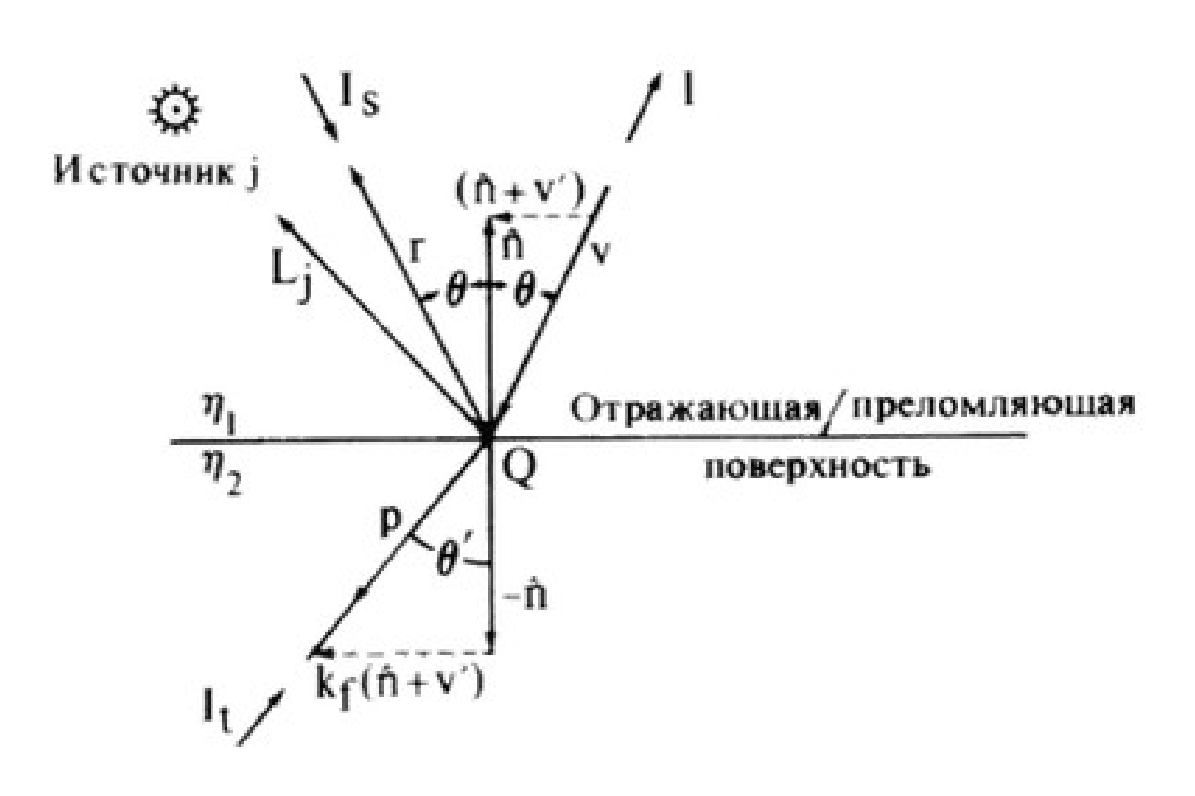
\includegraphics[width=0.7\linewidth]{whitted}
	\caption{Модель освещения Уиттеда}
	\label{whitted}
\end{figure}

В данной модели луч V, падающий на поверхность в точке Q, отражается в
направлении r и, если поверхность прозрачна, преломляется в направлении p. Тогда наблюдаемая интенсивность $I$ выражается формулой:

\begin{equation}\label{whitted_eq}
	I = k_a I_a + k_d \sum_{j} I_{l_j} (N; L_j) + k_s \sum_{j} I_{l_j} (S; R_j)^n + k_s I_s + k_t I_t,
\end{equation}
где $k_a$ - коэффициент рассеянного отражения,\\
\text{~~~~~}$k_d$ - коэффициент диффузного отражения,\\
\text{~~~~~}$k_s$ - коэффициент зеркального отражения,\\
\text{~~~~~}$k_t$ - коэффициент пропускаяния,\\
\text{~~~~~}$I_t$ - интенсивность света, падающего в точку Q по направлению p;\\
\text{~~~~~}$I_s$ - интенсивность света, падающего в направлении r и зеркально отраженного к наблюдателю в точке Q;\\
\text{~~~~~}$N$ - нормаль к поверхности в точке Q,\\
\text{~~~~~}$L_j$ - направление на $j$-ый источник света,\\
\text{~~~~~}$S$ и $R$ - локальные векторы наблюдения отражения,\\
\text{~~~~~}$n$ - степень пространственного распределения Фонга.

Для вычисления интенсивности преломленного света можно применить
закон Бугера-Ламберта-Бера для учета поглощения энергии при прохождении луча
света через вещество:

\begin{equation}\label{blb}
	I_t = I_0 e^{-k_{\lambda} l},
\end{equation}
где $I_0$ - интенсивность света на входе в вещество,\\
\text{~~~~~}$l$ - толщина слоя вещества, через который прошел свет;\\
\text{~~~~~}$k_{\lambda}$ - показатель поглощения.

Для данной работы была выбрана модель освещения Уиттеда, так как она
позволяет учесть такие оптические явления, как отражение и преломление света,
что позволит нам получать более реалистичное изображения, чем модели
Ламберта и Фонга.

\section*{Вывод}

В данном разделе были рассмотрены методы и алгоритмы, необходимые для написания программного обеспечения. Для описания объекта была выбрана модель полигональной сетки. Для представления поверхности слайма был выбран список граней, при этом информация о сетке будет храниться с помощью списка граней. Для физического моделирования слайма была выбрана модель масс с пружинами. В качестве алгоритма удаления невидимых ребер и поверхностей была выбрана обратная трассировка лучей. Для учета освещения была выбрана глобальная модель Уиттеда.

\clearpage
